\newpage
	\subsection{Quadratur nach Romberg}
	
	\defi{
		\n 
		Quadratur nach Romberg kombiniert zwei Trapezsummen unterschiedlicher Schrittweiten, um das exakte Ergebnis besser zu approximieren. Wir können das iterativ mit jeweils zwei und insgesamt mehr als zwei Trapezsummen machen, um eine höhere Genauigkeit zu erhalten.
		\n
		Wir konstruieren uns dafür Trapezsummen mit immer kleinerem $h$ bzw. größerem $N$, die wir auch inkrementell bestimmen können. Es gilt nämlich:
		\begin{align}
			\QTS(f;h) = \frac{\QTS(f; 2h)}{2} + h \cdot \l(f_1 + f_3 + \dots + f_{N-3} + f_{N-1} \r)
		\end{align}
		Die Romberg-Quadratur ist im Grunde eine \fat{Extrapolation}. Mithilfe der Kombination von Trapezsummen schätzt die Romberg-Quadratur den Wert an der Stelle $h=0$ ab, was im Prinzip dem analytischen Ergebnis entsprechen sollte (schrittweite von 0 wäre ja theoretisch die perfekte Approximation).
		\begin{figure}[H]
			\centering
			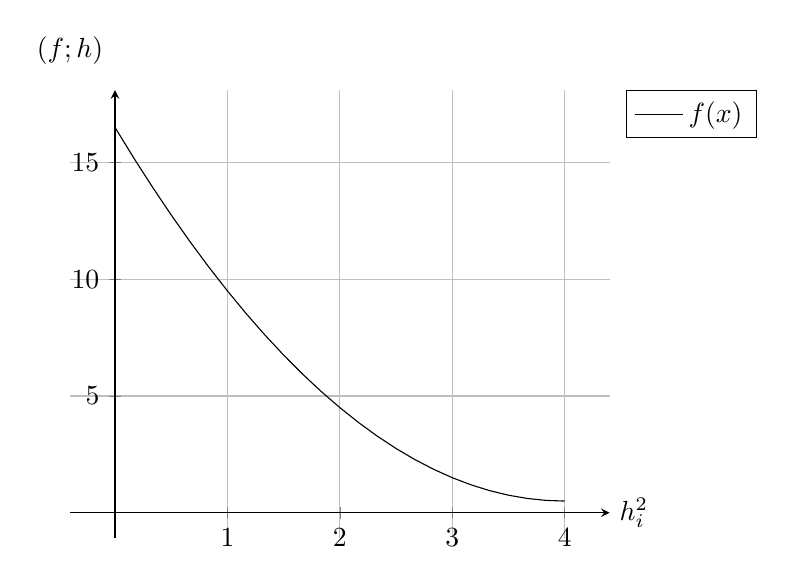
\begin{tikzpicture}
			\begin{axis}[
			axis lines=middle,
			xlabel=$h_i^2$,
			ylabel=$\QTS(f; h)$,
			enlargelimits,
			grid=major,
			%ytick={0,0.5,1},
			legend pos=outer north east,
			every axis x label/.style={at={(current axis.right of origin)},anchor=west},
			every axis y label/.style={at={(current axis.north west)},above=2mm},
			]
			\addplot[domain=0:4] {x^2 - 8*x + 16.5} node[left]{};
			\tikzPointUp{}{4,0.5}
			\tikzPointUR{}{2,4.5}
			\tikzPointUR{}{1,9.5}
			\tikzPointRight{}{0,16.5}
			\legend{$f(x)$}
			\end{axis}
			\end{tikzpicture}
			\caption{Die rechten drei Punkte sind hier die Werte von drei Trapezsummen. Durch diese kann der Punkt an der Stelle $h^2 = 0$ abgeschätzt werden. Das ist dann das Ergebnis der Romberg-Quadratur.}
		\end{figure}
	}

	\newpage
	\methode{\n
		Zum Kombinieren können wir ähnlich dem Newton und Aitken-Neville Verfahren eine Tabelle schreiben, die nach \fat{rechts unten} determiniert.
		\begin{table}[H]
			\label{table:romberg}
			\centering
			\begin{tabular}{cc|cccc}
				\toprule
				$h_k$  & $k$ & $Q_{k0}$ & $Q_{k1}$ & \dots & $Q_{kn}$ \\ \midrule
				$\frac{b-a}{1}$ & $0$ & $\QTS(f;\frac{b-a}{1}) = Q_{00}$ &  & & \\
				$\frac{b-a}{2}$ & $1$ & $\QTS(f;\frac{b-a}{2}) = Q_{10}$ & $Q_{11}$ &  & \\
				$\frac{b-a}{4}$ & $2$ & $\QTS(f;\frac{b-a}{4}) = Q_{20}$ & $Q_{21}$ & $Q_{22}$ & \\
				\vdots & & \vdots & & & $\ddots$ \\
			\end{tabular}
			\caption{Tabelle zum ausrechnen}
		\end{table}
		\noindent Mit folgender Gleichung kombinieren wir zwei beliebige Trapezsummen $\QTS(f, h_1)$ und $\QTS(f, h_2)$:
		\begin{align} 
 			\QTS(f, h_{\text{neu}}) = \QTS(f, h_2) + \frac{\QTS(f, h_2) - \QTS(f, h_1)}{\l(\frac{h_1^2}{h_2^2}\r) - 1} 
 		\end{align}	
		Informell und direkt auf das Dreiecksschema angepasst:
		\begin{align} 
 			Q_{\text{neu}} = Q\uleft + \frac{Q\uleft - Q\uleftUp}{\l(\frac{h\uleftUpDiagonal}{h\uleft}\r)^2 - 1} 
 		\end{align} 
 		Von der Notation her wie bei Newton-Verfahren (siehe \refChapter{chap:newtoninterpolation}), nur halt jetzt mit "links" statt "rechts" und anstelle von "unten" ist es halt darüber, also "oben".
	}

	\newpage
	\bsp{
		\n 
		% x^2 - 4
		Wir möchten folgende Berechnung annähern:
		\begin{align*} 
 			\int_{1}^{3}f(x) \d x
		\end{align*}
		Folgende Stützpunkte seien bekannt:
		\begin{table}[H]
			\label{table:ex_romberg}
			\centering
			\begin{tabular}{rccccc}
				\toprule
				$x$   	& $1$ 	& $1.5$ 	& $2$ 	& $2.5$		& $3$ \\ \midrule
				$f(x)$ 	& $-3$ 	& $-1.75$ 	& $0$   & $2.25$ 	& $5$    \\
				\bottomrule
			\end{tabular}
		\end{table}
		Damit können wir Romberg-Quadratur bis zu drei Trapezsummen aufstellen:
		\begin{table}[H]
			\label{table:ex_romberg_table}
			\centering
			\begin{tabular}{cc|ccc}
				\toprule
				$h_k$  & $k$ & $Q_{k0}$ & $Q_{k1}$ & $Q_{k2}$ \\ \midrule
				$\frac{b-a}{1}$ & $0$ & $\QTS(f;\frac{b-a}{1}) = Q_{00}$ &  & \\
				$\frac{b-a}{2}$ & $1$ & $\QTS(f;\frac{b-a}{2}) = Q_{10}$ & $Q_{11}$ &  \\
				$\frac{b-a}{4}$ & $2$ & $\QTS(f;\frac{b-a}{4}) = Q_{20}$ & $Q_{21}$ & $Q_{22}$
			\end{tabular}
		\end{table}
		\begin{align*} 
 			\QTS&(f;h) = h \cdot (\frac{f_0}{2} + f_1 + ... + f_{N-1} + \frac{f_N}{2}) \\
 			Q_{00} &= \QTS(f, \frac{b-a}{1}) = \QT(f) = 2 \cdot \frac{f(1) + f(3)}{2} = 2 \cdot \frac{-3 + 5}{2} = 2 \\
 			Q_{10} &= \QTS(f, \frac{b-a}{2}) = \QTS(f, 1) = 1 \cdot (\frac{-3}{2} + 0 + \frac{5}{2}) = 1 \\
			Q_{20} &= \QTS(f, \frac{b-a}{4}) = \QTS(f, 0.5) = 0.5 \cdot (\frac{-3}{2} - 1.75 + 0 + 2.25 + \frac{5}{2}) = 0.75 
 		\end{align*}
%		Tragen wir ein, was wir wissen:
%				$h_k$  & $k$ & $Q_{k0}$ & $Q_{k1}$ & $Q_{k2}$ \\ \midrule
%				$2$ & $0$ & $2$ &  & \\
%				$1$ & $1$ & $1$ & $Q_{11}$ &  \\
%				$0.5$ & $2$ & $0.75$ & $Q_{21}$ & $Q_{22}$ \\
		Jetzt geht es an das Kombinieren mit der Formel:
		\begin{align*} 
 			Q_{\text{neu}} &= Q\uleft + \frac{Q\uleft - Q\uleftUp}{\l(\frac{h\uleftUpDiagonal}{h\uleft}\r)^2 - 1}  \\
			Q_{11} &= 1 + \frac{1 - 2}{(\frac{2}{1})^2 - 1} = \frac{2}{3} \\
			Q_{21} &= 0.75 + \frac{0.75 - 1}{(\frac{1}{0.5})^2 - 1} = \frac{8}{12} 
 		\end{align*}
		\begin{table}[H]
			\label{table:ex_romberg_table3}
			\centering
			\begin{tabular}{cc|ccc}
				\toprule
				$h_k$  & $k$ & $Q_{k0}$ & $Q_{k1}$ & $Q_{k2}$ \\ \midrule
				$2$ & $0$ & $2$ &  & \\
				$1$ & $1$ & $1$ & $\nicefrac{2}{3}$ &  \\
				$0.5$ & $2$ & $0.75$ & $\nicefrac{8}{12}$ & $Q_{22}$ \\
			\end{tabular}
		\end{table}
		Jetzt noch das Ergebnis ausrechnen:
		\begin{align*} 
 			Q_{22} = \frac{8}{12} + \frac{\frac{8}{12} - \frac{2}{3}}{(\frac{2}{0.5})^2 - 1} = \frac{8}{12} + \frac{\frac{8}{12} - \frac{8}{12}}{16 - 1} = \frac{8}{12} = \frac{2}{3} 
 		\end{align*}
		In diesem Fall ist das Ergebnis schon exakt, da die unbekannte Funktion $f$ in Wahrheit $f(x) = x^2 - 4$ ist und die Fläche von $1$ bis $3$ analytisch exakt $\frac{2}{3}$ entspricht.
		\begin{figure}[H]
			\centering
			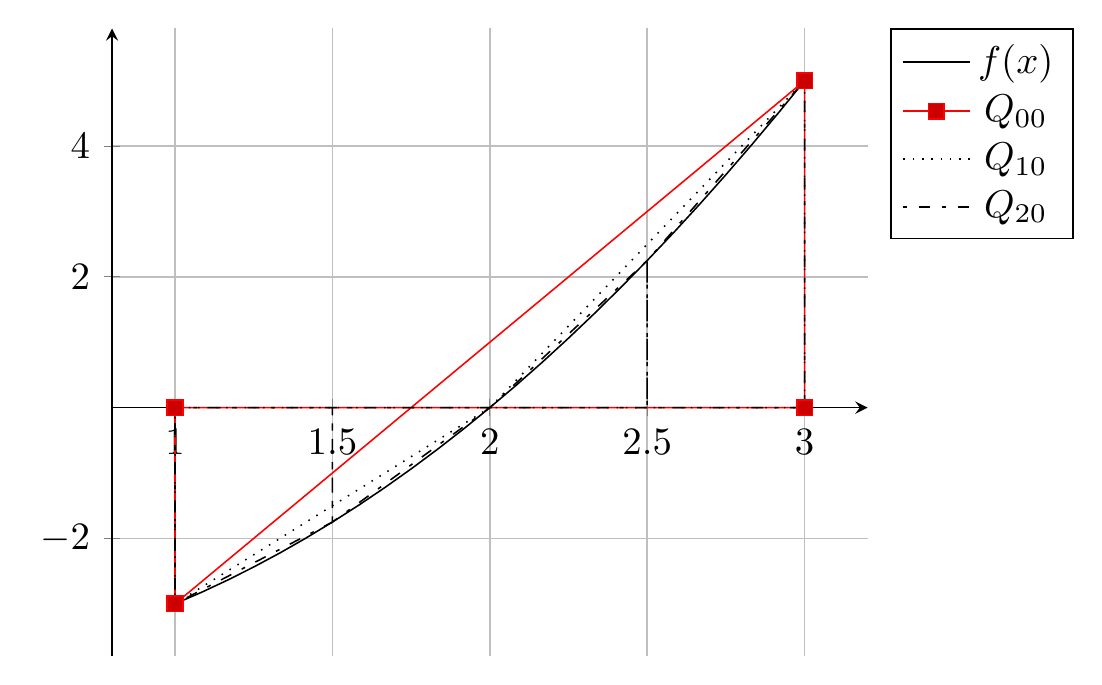
\begin{tikzpicture}[scale=1.4]
				\begin{axis}[
					axis lines=middle,
					xlabel=,
					ylabel=,
					enlargelimits,
					grid=major,
					%ymax=3.1,
					%ymin=-0.5,
					legend pos=outer north east,
					]
					\addplot[domain=1:3] {x^2 - 4} node[left]{};
					\addplot coordinates {
						(1, 0)
						(1, -3)
						(3, 5)
						(3, 0)
						(1, 0)
					};
					\addplot[dotted] coordinates {
						(1, 0)
						(1, -3)
						(2, 0)
						(3, 5)
						(3, 0)
						(1, 0)
					};
					\addplot[dash pattern=on 1pt off 3pt on 3pt off 3pt] coordinates {
						(1, 0)
						(1, -3)
						(1.5, -1.75)
						(1.5, 0)
						(1.5, -1.75)
						(2, 0)
						(2.5, 2.25)
						(2.5, 0)
						(2.5, 2.25)
						(3, 5)
						(3, 0)
						(1, 0)
					};
					\legend{$f(x)$,$Q_{00}$, $Q_{10}$, $Q_{20}$}
				\end{axis}
			\end{tikzpicture}
			\caption{Die verschiedenen Trapezsummen, die wir in dem Beispiel genutzt haben sowie die exakte Funktion.}
		\end{figure}
	}